\documentclass[10pt, landscape]{article}
\usepackage[scaled=0.92]{helvet}
\usepackage{calc}
\usepackage{multicol}
\usepackage{ifthen}
\usepackage[a4paper,margin=5mm,landscape]{geometry}
\usepackage{amsmath,amsthm,amsfonts,amssymb}
\usepackage{color,graphicx,overpic}
\usepackage{hyperref}
\usepackage{newtxtext} 
\usepackage{enumitem}
\usepackage{amssymb}
\usepackage[table]{xcolor}
\usepackage{vwcol}
\usepackage{tikz}
\usetikzlibrary{arrows.meta}
\usetikzlibrary{calc}
\usepackage{mathtools}
\usepackage{nicematrix}
\usepackage[T1]{fontenc} %%% <--- NOTE THIS
% for relations
\usepackage{cancel}
\usepackage{ mathrsfs }
\usepackage{listings}
\usepackage{background}
\setlist{nosep}

\usepackage{etoolbox}
\makeatletter
\preto{\@verbatim}{\topsep=0pt \partopsep=0pt }
\makeatother

\backgroundsetup{
scale=1,
color=black,
opacity=0.2,
angle=0,
contents={%
  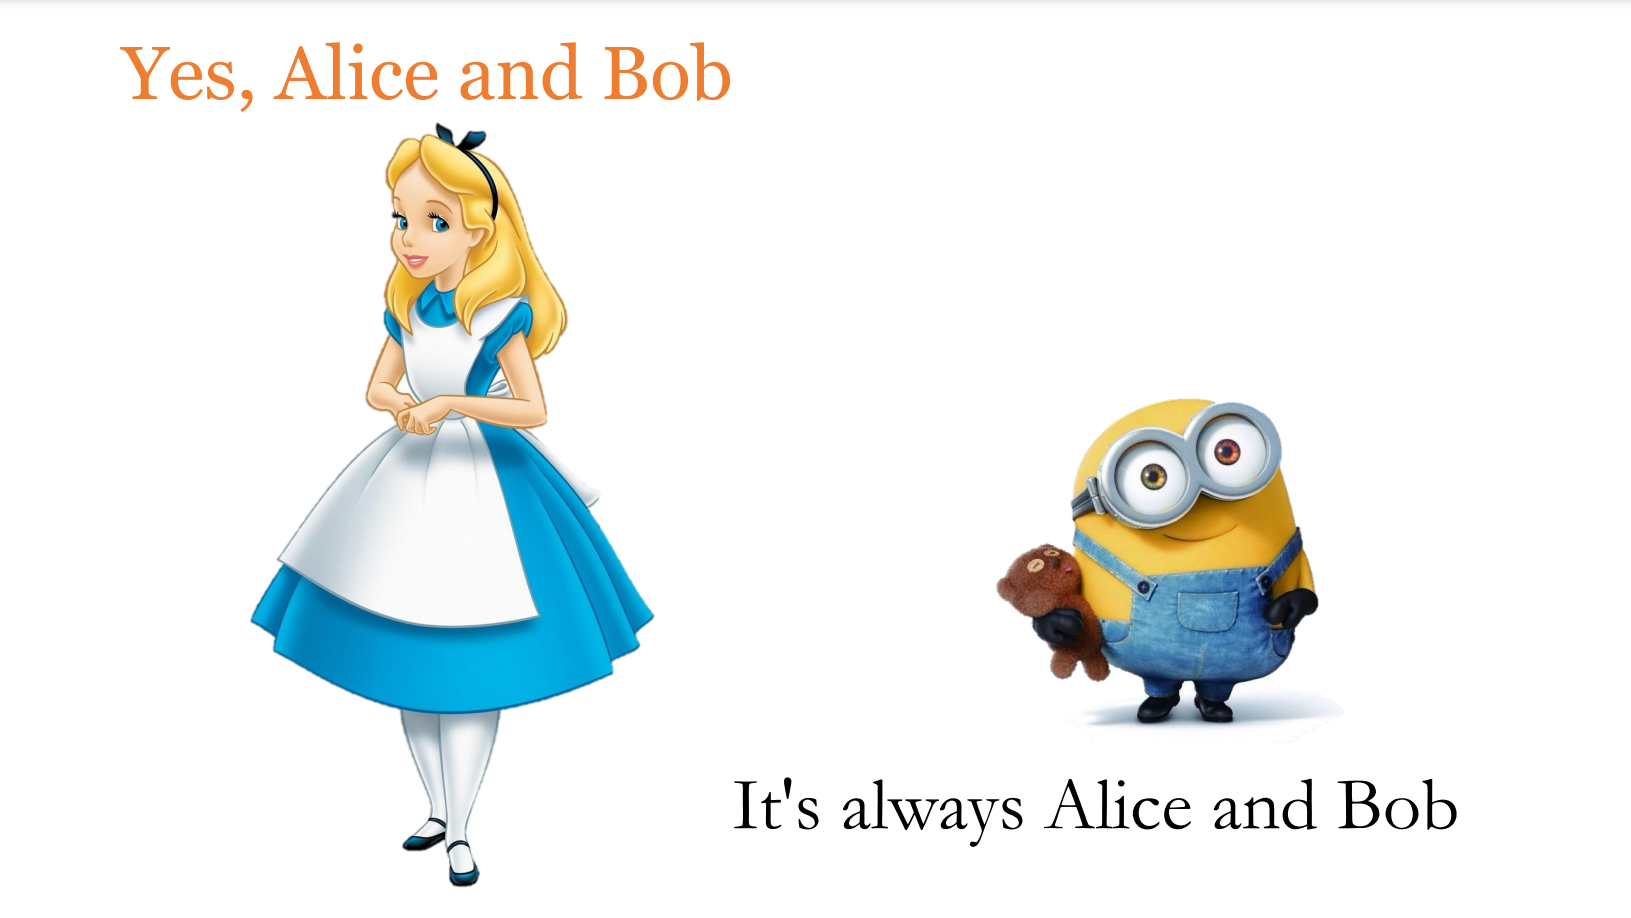
\includegraphics[width=\paperwidth,height=\paperheight]{alice.png}
  }%
}

\pdfinfo{
  /Title (CS2105.pdf)
  /Creator (TeX)
  /Producer (pdfTeX 1.40.0)
  /Author (Seamus)
  /Subject (Example)
  /Keywords (pdflatex, latex,pdftex,tex)}

\lstset{language=Java,keywordstyle={\bfseries \color{black}}}

% Turn off header and footer
\pagestyle{empty}

\newenvironment{tightcenter}{%
  \setlength\topsep{0pt}
  \setlength\parskip{0pt}
  \begin{center}
}{%
  \end{center}
}

% redefine section commands to use less space
\makeatletter
\renewcommand{\section}{\@startsection{section}{1}{0mm}%
                                {-1ex plus -.5ex minus -.2ex}%
                                {0.5ex plus .2ex}%x
                                {\normalfont\large\bfseries}}
\renewcommand{\section}{\@startsection{section}{2}{0mm}%
                                {-1explus -.5ex minus -.2ex}%
                                {0.5ex plus .2ex}%
                                {\normalfont\normalsize\bfseries}}
\renewcommand{\subsection}{\@startsection{subsection}{3}{0mm}%
                                {-1ex plus -.5ex minus -.2ex}%
                                {1ex plus .2ex}%
                                {\normalfont\small\bfseries}}%
\renewcommand{\familydefault}{\sfdefault}
\renewcommand\rmdefault{\sfdefault}
% makes nested numbering (e.g. 1.1.1, 1.1.2, etc)
\renewcommand{\labelenumii}{\theenumii}
\renewcommand{\theenumii}{\theenumi.\arabic{enumii}.}
\renewcommand\labelitemii{•}
%  for logical not operator
\renewcommand{\lnot}{\mathord{\sim}}
\renewcommand{\bf}[1]{\textbf{#1}}
\newcommand{\abs}[1]{\vert #1 \vert}
\newcommand{\Mod}[1]{\ \mathrm{mod}\ #1}

\makeatother
\definecolor{myblue}{cmyk}{1,.72,0,.38}
\everymath\expandafter{\the\everymath \color{myblue}}
% Define BibTeX command
\def\BibTeX{{\rm B\kern-.05em{\sc i\kern-.025em b}\kern-.08em
    T\kern-.1667em\lower.7ex\hbox{E}\kern-.125emX}}
\let\iff\leftrightarrow
\let\Iff\Leftrightarrow
\let\then\rightarrow
\let\Then\Rightarrow

% Don't print section numbers
\setcounter{secnumdepth}{0}

\setlength{\parindent}{0pt}
\setlength{\parskip}{0pt plus 0.5ex}
%% this changes all items (enumerate and itemize)
\setlength{\leftmargini}{0.5cm}
\setlength{\leftmarginii}{0.5cm}
\setlist[itemize,1]{leftmargin=2mm,labelindent=1mm,labelsep=1mm}
\setlist[itemize,2]{leftmargin=4mm,labelindent=1mm,labelsep=1mm}

%My Environments
\newtheorem{example}[section]{Example}
% -----------------------------------------------------------------------

\begin{document}
\raggedright
\footnotesize
\begin{multicols*}{3}

% multicol parameters
% These lengths are set only within the two main columns
\setlength{\columnseprule}{0.25pt}
\setlength{\premulticols}{1pt}
\setlength{\postmulticols}{1pt}
\setlength{\multicolsep}{1pt}
\setlength{\columnsep}{2pt}

\begin{center}
    \fbox{%
        \parbox{0.8\linewidth}{\centering \textcolor{black}{
            {\Large\textbf{CS2105}}
            \\ \normalsize{AY24/25 Sem 2}}
            \\ {\footnotesize \textcolor{myblue}{by ngmh}} 
        }%
    }
\end{center}

\section{Introduction}
\begin{itemize}
    \item The Internet is a network of connected computing devices / hosts that run network applications which talk to each other with protocols
    \item Hosts access the Internet through access networks
    \item Circuit-Switching: Dedicated end-end resources reserved between source and destination
    \item Packet-Switching (e.g. Internet): Host breaks message down into packets which are passed from one router to the next
    \item Transmission delay $=packet \ length/transmission\ rate$
    \item Internet is a Network of Networks
    \item Protocol Layers: Application, Transport (Process-Process), Network (Routing of datagrams from host to host, Link (Data transfer between neighbouring network elements), Physical (Bits on the wire)
\end{itemize}

\section{Delay and Loss}
\begin{itemize}
    \item Packets queue in router buffers to be sent out, might be dropped if capacity is reached
    \item Processing Delay: Time to check bit errors, and determine output link
    \item Queueing Delay: Time waiting in queue for transmission
    \item Transmission Delay: $L/R$, time for packet to be fully sent out
    \item Propagation Delay: $d/s$, time for packet to travel across physical link
    \item End-End Delay is the sum of these four factors
    \item $traceroute$ displays path from source to destination by sending a series of small packets with different TTL
    \item Throughput: How many bits can be transmitted per unit time
    \item 1 byte = 8 its, Micro, Milli, Standard, Kilo, Mega, Giga, Tera, B = bytes, b = bits
\end{itemize}

\section{Application Layer}
\begin{itemize}
    \item Client-Server Architecture: Server waits for incoming requests and provides service to clients who initiate contact
    \item P2P Architecture: No dedicated server, end systems communicate with each other, highly scalable but difficult to manage
    \item Serivce Criteria:
    \begin{itemize}
        \item Data Integrity: Can app tolerate data loss e.g. file transfer v/s audio streaming
        \item Throughput: How much bandwidth does the app need e.g. multimedia
        \item Timing: Is the app time sensitive e.g. online games
        \item Security: Does the app need encryption and data integrity
    \end{itemize}
    \item Process Identification:
    \begin{itemize}
        \item IP Address: Globally unique, identifies host, IPv4 is 32 bits split into 4 bytes in dotted decimal, IPv6 is 128 bits split into 8 sets of 2 bytes in : hexadecimal
        \item Port Number: Locally unique, identifies process, 16 bit number
    \end{itemize}
\end{itemize}

\section{HTTP}
\begin{itemize}
    \item HyperText Markup Language (HTML): What
    \item Uniform Resource Locator (URL): Where
    \item HyperText Transfer Protocol (HTTP): How
    \item A webpage has a base HTML file and other referenced objects with their own URLs
    \item Uses TCP as a transport service
    \item RTT: Time for a packet to travel from client to server and back
    \item HTTP/1.0: New connection established for each resource, time taken is $2RTT+transmission\ time$ for each
    \item HTTP/1.1: Pipelining: New request is made before receiving response of old requests as soon as resource is encountered
    \item HTTP/1.1 Persistence: Connection left open after sending response, subsequent messages use the same connection
    \item HTTP/2 Multiplexing: Response can come back in any order, even partially
    \item Request:
\begin{verbatim}
    GET /~cs2105/demo.html HTTP/1.1\r\n
    Host: www.comp.nus.edu.sg\r\n
    User-Agent: Mozilla/5.0\r\n
    Connection: close\r\n
\end{verbatim}
    \item Response:
\begin{verbatim}
    HTTP/1.1 200 OK\r\n
    Date: Wed, 01 Jul 201508:47:52 GMT\r\n
    Connection: Keep-Alive\r\n
    Content-Length: 73\r\n
    Content-Type: text/html\r\n
    Keep-Alive: timeout=5, max=100\r\n
    \r\n
    <!DOCTYPE html>...
\end{verbatim}
    \item Status Codes: 200 OK, 301 Moved Permanently, 304 Not Modified, 403 Forbidden, 404 Not Found, 500 Internal Server Error
    \item HTTP is stateless, and uses cookies in messages to maintain state
    \item Caching: Don't send object if client has up-to-date version of resource, check using If-modified-since header which can give 304
\end{itemize}

\section{Domain Name System (DNS)}
\begin{itemize}
    \item Translates between hostname and IP address
    \item Stored as resource records with different types (A = address, NS = nameserver, CNAME = canonical name, MX = mail exchange)
    \item Use nslookup or dig to find information
    \item Stored in distributed hierarchical databases, 13 root nameservers worldwide
    \item Top-level domain (TLD) servers: Responsible for domain suffixes and country domains
    \item Authoritative servers: Organisation's own DNS servers, provides mappings for oganisation's named hosts
    \item Local DNS Server: Does not belong to hierarchy, each ISP has one
    \item Recursive Query: DFS style query
    \item Iterative Query: BFS style, requests all come from local DNS server
    \item DNS Caching: Mapping is cached once nameserver leans about it, have TTL
    \item Runs over UDP/53
\end{itemize}

\section{Sockets / Transport Layer}
\begin{itemize}
    \item Host runs applicaitons in multiple processes, which are top-level execution containers with independent memory space
    \item Threads run in a process and share the same memory
    \item Identified by IP Address and Port Number
    \item Sockets are the abstraction interface between processes in the application layer and transport layer protocols
    \item Datagram Socket:
    \begin{itemize}
        \item Uses UDP, only one socket is needed
        \item Each application creates a packet with recipient and OS attached return information
    \end{itemize}
    \item Stream Socket:
    \begin{itemize}
        \item Uses TCP, where connection is established between two processes
        \item Data flows in continuous streams, separated into client and server, does not need to attach address information
        \item Server creates welcome socket, and forks a new socket when contacted by a client
        \item Client creates a socket to establish connection with server, and each connection has its own socket instance
    \end{itemize}
\end{itemize}

\section{Reliable Protocols / Delivery Transfer}
\begin{itemize}
    \item Transport layer resides on end hosts and provides process-process communication
    \item Network layer provides host-host, best-effort, and unreliable communication
    \item Unreliable channel might corrupt / drop / re-order / delay packets
    \item rdt 1.0: Reliable channel, no special handling needed
    \item rdt2.0: Channel with bit errors, use checksum to detect
    \item Requires ACK and NAK as well as retransmissions, but fails if acknowledgment gets corrupted
    \item rdt2.1: Add sequence number to handle duplicates, retransmits if acknowledgment is corrupted
    \item rdt2.2: Replace NAK with ACK of last correctly received packet
    \item rdt3.0: Packet can be lost, corrupted, or delayed, retransmits ACK or packet on timeout
    \item Utilisation: Fraction of time link is actually being used, $U=\frac{time \ sending}{total\ time}=\frac{d_{trans}}{d_{trans}+RTT}$
    \item Throughput: $\frac{L}{RTT+d_{trans}}$
    \item Pipelining allows multiple packets to be transmitted at once, requires buffering, increases utilisation
    \item Go-Back-N:
    \begin{itemize}
        \item Cumulative ACK, ACK $n$ means all packets $\leq n$ have been received
        \item Keeps track of $n$ unACKed packets, with timer for oldest one
        \item On timeout, retransmit all packets, receiver ignores out of order packets
    \end{itemize}
    \item Selective Repeat:
    \begin{itemize}
        \item Each packet has a timer, and is retransmitted on timeout
        \item Receiver individually acknowledges correctly received packets, buffering out of order packets
        \item Has overhead from maintaining timers
    \end{itemize}
\end{itemize}

\section{User Datagram Protocol (UDP)}
\begin{itemize}
    \item Adds very little on top of IP
    \item Unreliable tranmission, requires RDT, no flow or congestion control
    \item No connection setup or state needed, faster and less resources needed
    \item Less overhead due to small header size, no congestion control
    \item Multiplexing: Allow multiple sockets to send data on the same transmission channel to the same socket
    \item Transport layer de-multiplexes using destination port number, directs it to correct UDP socket
    \item Checksum: 16-bits used to identify single bit flips
    \item Split segment into 16-bit integers, add with wrap around carry, then compute 1s complement
    \item At receiver, perform the same addition with checksum which should result with all bits set
\end{itemize}
\begin{center}
    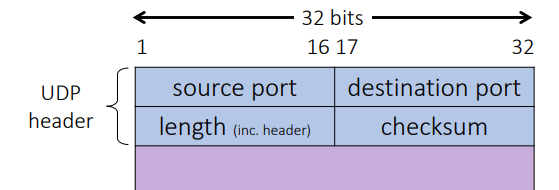
\includegraphics[width=0.9\linewidth]{UDP.png}
\end{center}

\section{Transmission Control Protocol (TCP)}
\begin{itemize}
    \item Connection-oriented, handshake must be established
    \item Reliable, in-order byte stream, segments have Maximum Segment Size (MSS) not including header
    \item Has flow control and congestion control
    \item Socket is identified by source and destination IP address and port
    \item Guaranteed delivery, but no guarantee on throughput or reliability
    \item Sequence Number: Byte number of first byte of data in segment
    \item Acknowledgment Number: Sequence number of next byte of data expected, cumulative ACK
    \item TCP Timeout Value: Too short causes retransmissions, too long causes slow reaction to loss
    \item Estimate RTT: Take Sample RTT and use it to calculate Estimated RTT
    \item $RTT_E=(1-\alpha)RTT_E+\alpha RTT_S$, typically $\alpha=\frac{1}{8}$, exponential weighted moving average
    \item Set retransmission timeout based on deviation of RTT and safety margin
    \item $RTT_{dev}=(1-\beta)RTT_{dev}+\beta |RTT_S-RTT_E|$, typically $\beta=\frac{1}{4}$
    \item $RTO=RTT_E+4RTT_{dev}$
    \item Fast Retransmission: Resend immediately upon receiving 3 duplicate ACKs
    \item Connection is established using 3-way handshake: Sender sends TCP SYN and initial sequence number, server chooses initial sequence number and sends TCP SYN/ACK, client sends ACK and data
    \item Half-Open Connections: Vulnerable to SYN flooding or SYN/ACK flooding DoS
    \item Each side closes own side of connection, sends segments with FIN bit, can only receive data after sending it
    \item Flow Control: Receiver buffers data to application, telling sender how much data it can send, sender sends 0-data segment when buffer empties
\end{itemize}
\begin{center}
    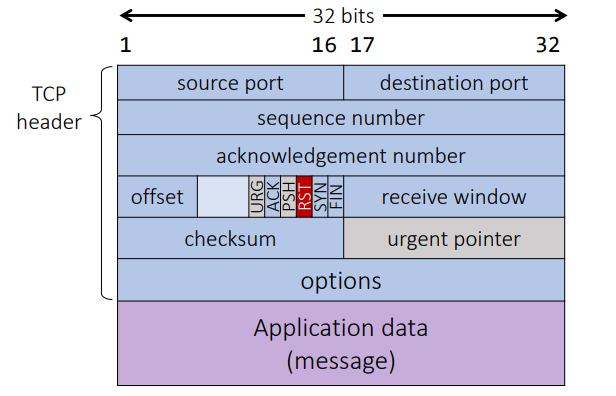
\includegraphics[width=0.9\linewidth]{TCP.png}
\end{center}

\section{Network Layer}
\begin{itemize}
    \item Provides communication service between any two hosts in the world
    \item Each host needs to be addressed
    \item Path between all pairs of hosts needs to be determined
    \item Need to define a protocol / service guarantee
    \item Router: Device that forwards packets between networks
\end{itemize}

\section{Network Addresses}
\begin{itemize}
    \item IP Address: used to identify every interface of host, has to be globally unique, 32 bits
    \item Routers store forwarding tables with destination IP addresses and output links
    \item Address Aggregation: Use wildcards to specify range of addresses to reduce size of forwarding table
    \item Subnet: Network formed by a group of interconnected hosts which can reach each other without a router, single link between 2 routers also counts as a subnet
    \item IP Address is made up of network / subnet prefix and host ID, given in a.b.c.d/x where x is number of bits in subnet prefix
    \item Subnet Mask is used to determine which subnet an IP address belongs to
    \item ISPs own a consecutive block of IP addresses
    \item There are some special IP addresses, such as localhost, private, and broadcast addresses
\end{itemize}

\section{Network Address Translation (NAT)}
\begin{itemize}
    \item Public Addresses: Globally unique and routable
    \item Private IP Addresses: Not globally unique or routable, used within organisations
    \item WAN: The Internet, LAN: Local network
    \item All datagrams leaving local network through router have same source NAT IP address
    \item Within local network, hosts have own private IP addresses
    \item NAT translation table: Translates WAN side addresses and ports to LAN side addresses and ports
    \item Router replaces datagram information as necessary
    \item Easier to change addresses, and hosts within network are not visible to outside world
    \item Port number is 16-bit, NAT supports $2^{16}$ addresses
\end{itemize}

\section{IPv4 Fragmentation}
\begin{itemize}
    \item Datgram: Ver is protocol version number, IP datagram length includes header, TTL is decremented at each hop, 20 bytes total
\end{itemize}
\begin{center}
    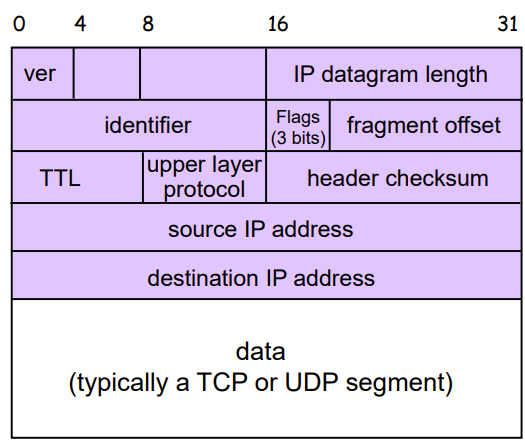
\includegraphics[width=0.9\linewidth]{IP.png}
\end{center}
\begin{itemize}
    \item Different links have different Maximum Transfer Units (MTU), maximum amount of data a link-level frame can carry
    \item IP Datagrams that are too large might be fragmented by routers to be reassembled at destination
    \item Uses identifier, flags, and fragment offset fields in header
    \item Each fragment shares the same identifier
    \item Flag is 1 if there is next segment, and 0 at last segment
    \item Offset is in units of 8 bytes, relative to beginning of original datagram
\end{itemize}

\section{Dynamic Host Configuration Protocol (DHCP)}
\begin{itemize}
    \item Allocates IP addresses to hosts in network, renewable and reusable
    \item Runs over UDP, Server Port: 67, Client Port: 68
    \item Host broadcasts DHCP discover, Server responds with DHCP offer, Host request IP address DHCP request, Server sends address DHCP ACK
    \item Destination is broadcast address with correct port, original host IP is 0
\end{itemize}

\section{Routing}
\begin{itemize}
    \item Look for longest prefix match in forwarding table ,and forward to corresponding link
    \item Routing: Finding least cost path between two vertices in graph, but every node only has information about immediate neighbours
    \item $C_{x, y}$: cost of link between $x$ and $y$, $D_x(y)$: least-cost path from $x$ to $y$
    \item Bellman-Ford: $D_\alpha(z)=min_{a\in N}\{c(\alpha, a)+D_a(z)\}$, min is taken over all direct neighbours $a$ of $\alpha$
    \item Distance Vector Algorithm:
    \item Each neighbour sends its distance vector to source telling it cost from self to target
    \item At each time period, all nodes receive the distance vectors from neighbours and compute their new local distance vector before sending it out
    \item Iterative, asynchronous, distributed, self-stopping when no updates
    \item Routing Information Protocol implements DV, using hop count as the cost metric, exchanging every 30 seconds over UDP/520
    \item Self-repair: Assume neighbour has failed after 3 minutes with no update
    \item Intra-AS routing: Find good path between two routers in same autonomous system, focuses on performance, uses RIP/OSPF
    \item Inter-AS routing: Handles interfaces between ASs, needs policy, uses BGP
\end{itemize}

\section{Internet Control Message Protocol (ICMP)}
\begin{itemize}
    \item Used by hosts and routers to communicate network-level information such as error reporting or echo requests and replies
    \item Messages carried in IP datagrams, starting after IP header
    \item Header consists of Type + Code (Sub type) + Checksum + Others
\end{itemize}

\section{Network Layer Services}
\begin{itemize}
    \item Delivers packets to receiving hosts, includes routing, IP, and ICMP
    \item Data plane: Local, per-router function, determines forwarding within router
    \item Control plane: Network-wide logic, determines how datagram is routed among routers on path between source and destination hosts
    \item Routers use longest prefix matching, performed using ternary content addressable memories (TCAMs), content addressable
    \item Best-effort basis
    \item Exists in every host and router, router examines header fields in all IP datagrams passing through it
\end{itemize}

\section{Link Layer}
\begin{itemize}
    \item Send data between $n$ nodes via cable
    \item Complete graph: Interconnect every pair of nodes, but each link needs to be addressed and not scalable
    \item Broadcast link: Shared link across multiple nodes, needs protocol, and error handling
    \item Sends datagrams between adjacent nodes over a single link
    \item IP datagrams are encapsulated in link-layer frames for transmission, and different links might use different protocols
    \item Possible services include framing, link access control, error detection and correction, and reliable delivery
    \item Link layer is implemented in an adapter / network interface card (NIC) on a chip
    \item Point-Point Link: Sender and receiver connected by dedicated link
    \item Broadcast Link: Shared medium, every node receives a copy of transmitted frames
\end{itemize}

\section{Multiple Access Protocols}
\begin{itemize}
    \item If two or more nodes transmit simultaneously, collision occurs
    \item Ideal protocol: Collision free, efficient, fair, and fully decentralised, coordination must use channel itself
\end{itemize}

\subsection{Random Access Protocols}
\begin{itemize}
    \item Nodes transmit at full speed with no prior coordination
    \item Protocol specifies how to detect collisions and recover from them
\end{itemize}

\subsubsection{ALOHA}
\begin{itemize}
    \item Slotted ALOHA: All frames have equal size, time is divided into slots of equal length of time to transmit 1 frame
    \item Nodes have synchronised time, transmitting only at beginning of a slot
    \item Node retransmit frame in each subsequent slot with probability $p$ if there is a failure
    \item Not collision free, and only efficient when one node is active, perfectly fair, decentralised
    \item Pure ALOHA: No time slots or synchronisation, nodes transmit frames immediately, waits for 1 frame transmission time before retransmission with probability $p$
    \item Not collision free, even less efficient, perfectly fair, decentralised
    \item Carrier Sense Multiple Access (CSMA): Listen before transmission, take note of other node's activity
    \item Defer transmission until channel is idle, but can still have collisions due to propagation delay
\end{itemize}

\subsubsection{Carrier Sense Multiple Access (CSMA)}
\begin{itemize}
    \item CSMA/CD (Collision Detection): In CSMA, node does not stop transmission even when collision is detected
    \item With CD, abort transmission on collision detection and retransmit after random delay
    \item Adapt retransmission attempts to estimated current load, so probability of collision decreases
    \item Binary Exponential backoff: After $m$ collision, choose $K$ at random from $\{0,..., 2^m-1\}$, with $p=\frac{1}{2^m}$ before waiting $K$ time units for retransmission (1 time unit is 512 bit transmission time for Ethernet)
    \item If frame size is too small, collision happens but cannot be detected, Ethernet uses 64B
    \item Can be avoided with $2max(d_{prop})\leq d_{trans}$, where $max(d_{prop})$ is directly proportional to the diameter of the network, and $d_{trans}$ is directly proportional to frame size
    \item CSMA(/CD) is not collision free, but is efficient, fair, and decentralised
\end{itemize}

\subsection{Taking-Turns Protocols}
\begin{itemize}
    \item Polling: One node is designated as master node, and polls each of the nodes in round-robin fashion, telling them how many frames they can transmit
    \item Collision free, efficient, fair, but not decentralised with a single point of failure
    \item Token Passing: Special frame is sequentially passed from one node to next, sequentially
    \item Node holds on to token if it has frames to transmit, and sends a maximum number of frames before passing it on
    \item Collision free, efficient, perfectly fair, and decentralised, but token loss is disruptive, and ring can be broken by failure
\end{itemize}
\subsection{Channel Partitioning Protocols}
\begin{itemize}
    \item Time Division Multiple Access (TDMA): Access channel in rounds, each node gets fixed length time slots in each round for data transmission
    \item Collision free, inefficient, perfectly fair and decentralised
    \item Frequency Division Multiple Access: Channel spectrum is divided into frequency bands, each node is assigned a fixed frequency band, unused transmission time in frequency bands go idle
    \item Collision free, inefficient, perfectly fair and decentralised
\end{itemize}

\section{Error Detection and Correction}
\begin{itemize}
    \item EDC: Error detection and correction bits
    \item Not totally reliable
    \item Single Bit: In even parity scheme, sender include one additional bit so that total number of 1s is even
    \item Can detect odd number of single bit errors, does not work well as errors are often clustered together
    \item 2-Dimensional: bits are divided into $i$ rows and $j$ columns, compute parity bit for each row and column and total parity bit
    \item Can detect and correct single bit errors, and detect two-bit errors
    \item Cyclic Redundancy Check: Generate $r$ bit error detection code for $d$ digit number
    \item Use $r+1$ bit number $G$, known as generator
    \item Send data appended with $r$ bit CRC
    \item Perform calculations modulo 2, same as XOR, repeatedly divide $D$ by $G$ to get $R$ for sender
    \item Receiver divides sender message by $G$, should get zero remainder
    \item Easy to implement, can detect all odd number of single bit errors, CRC of $r$ bits can detect all burst errors of up to $r$ bits, and all burst errors $>r$ bits with $p=1-0.5^r$
\end{itemize}

\section{Local Area Network (LAN)}
\subsection{Ethernet}
\begin{itemize}
    \item Network that interconnects computers within a geographical area
    \item Ethernet is the dominant wired LAN technology
    \item Ethernet Frame:
\end{itemize}

\begin{center}
    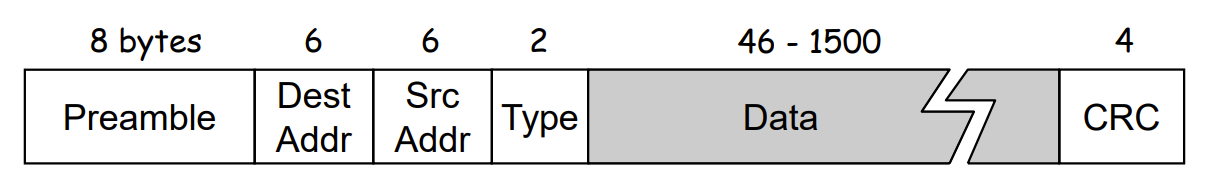
\includegraphics[width=0.9\linewidth]{eth.png}
\end{center}

\begin{itemize}
    \item Address are in Media Access Control (MAC) address
    \item If frame matches destination address or broadcast address, NIC passes it to network layer protocol, if not it discards it
    \item Size ranges from 46-1500 bytes, in line with MTU and minimum frame size
    \item Type Indiates higher layer protocol, allowing Ethernet to multiplex them
    \item Preamble starts with $AAAB$ in hex, and is used to synchronise receiver and sender clock rates, important if there is a long string of bits with the same value
    \item Ethernet is unreliable, and uses CSMA/CD
    \item Bus Topology: Broadcast LAN, all transmitted frames are received by all adapters connected to the bus, but single point of failure and slow
    \item Star Topology:
    \item Hub: Nodes are connected to hub, a physical-layer device that acts on individual bits rather than frames, cheaper but slow due to collisions
\end{itemize}
\subsection{Link Layer Switches}
\begin{itemize}
    \item Switch: Nodes are directly connected to a switch, which is a layer-2 device that works on frames rather than bits, store-and-forward, with no collisions
    \item Uses CSMA/CD to access link, is transparent, and plug-and-play (does not require configuration)
    \item Examines incoming frames MAC address and selectively forward to one or more outgoing links
    \item Nodes have dedicated direct connection to switch, which buffers packets
    \item Switch has a switch table which maps MAC address of host to interface to reach host, stored with TTL
    \item Switch learns which hosts can be reached when receiving a frame from sender, recording it in switch table
    \item When a frame is received:
    \begin{itemize}
        \item Record the incoming link and MAC address of sending host
        \item Index switch table using MAC destination address
        \item If entry is found, forward it to interface indicated only if destination on segment is different from which frame arrived
        \item If entry is not found, broadcast frame to all interfaces except arriving interface
    \end{itemize}
\end{itemize}

\subsection{Link Layer Addressing and ARP}
\begin{itemize}
    \item MAC Address: Every adapter has one, adapter uses it to check destination MAC address of frame and filters if necessary
    \item Typically 48 bits, burned in the Read-Only memory of an NIC, written in hexadecimal pairs, broadcast address is all 1s
    \item Each IP node has an Address Resolution Protocol (ARP) table, sorting mapping between IP address, MAC address, and TTL
    \item Sending within same subnet:
    \begin{itemize}
        \item If source knows destination MAC address from ARP table, create a frame with it and simply send it
        \item If not, broadcast an ARP query packet with destination IP address
        \item Only destination will reply with its MAC address, sent to source
        \item Source caches destination IP and MAC address mapping in ARP table
    \end{itemize}
    \item Sending to another subnet:
    \begin{itemize}
        \item Source creates IP datagram with source and destination IP addresses
        \item Source creates link layer datagram with router's MAC address as destination address, frame contains IP datagram
        \item Router removes link layer frame, and passes it to IP layer
        \item Router forwards datagram with IP addresses to receiving router
        \item Receiving router creates link layer frame with destination MAC address, containing original IP datagram, forwarding to destination
    \end{itemize}
\end{itemize}

\section{Network Security}
\begin{itemize}
    \item Intruders or eavesdroppers might edit messages
    \item Listen, delete / modify, add messages / impersonate
    \item Repudiation: Proving that transaction did not happen between two entities
    \item Confidentiality: Only sender and intended receiver should understand message contents
    \item Message Integrity: Sender and receiver want to ensure message is not altered without detection
    \item Authentication: Sender and receiver want to confirm identity of each other
\end{itemize}
\subsection{Confidentiality}
\begin{itemize}
    \item Cryptography: Allow a sender to disguise data so that intruder cannot gain information from it, while allowing receiver to recover original data from disguised data
    \item $m$: plaintext messsage
    \item $K_A(.)$: encryption algorithm with key $K_A$, $K_A(m)$: ciphertext
    \item $K_B(.)$: decryption algorithm with key $K_B$, $K_B(K_A(m))=m$
    \item Algorithms and keys are agreed upon beforehand, which can be symmetric or asymmetric
    \item Casesar Cipher: A substitution cipher where one thing is substituted for another, fixed shift of alphabet, only 25 possible keys
    \item Monoalphabetic Cipher: Substitute one letter for another, $26!$ mappings possible, but susceptible to dictionary attack or statistical analysis
    \item Attacks: Ciphertext only, known-plaintext (has plaintext corresponding to ciphertext), chosen-plaintext (can get ciphertext for chosen plaintext)
    \item Polyalphabetic Encryption: Compose multiple mappings on each other in a cyclic pattern for each character
    \item Block Cipher: Encrypt message in blocks of $K$ bits, use a one-to-one mapping to encode a block, $2^K!$ keys
    \item Data Encryption Standard: 56-bit symmetric key, 64-bit block, cracked in less than a day
    \item Advanced Encryption Standard: 128-bit blocks, with 128/192/256 bit keys, takes very very long to break
    \item Need many symmetric keys, one for each pair of individuals
\end{itemize}
\subsubsection{RSA}
\begin{itemize}
    \item Public Key Cryptography: Sender uses public encryption key known to all, receiver uses a private decryption key only known to them
    \item Requirements: Need $K_B^+(.)$ and $K_B^-(.)$ such that $m=K_B^-(K_B^+(m))$, and impossible to compute $K_B^-$ from $K_B^+$
    \item RSA Encryption:
    \begin{itemize}
        \item Choose two large prime $p, q$
        \item Compute $n=pq, z=(p-1)(q-1)$
        \item Choose $e<n$ which is relatively prime with $z$
        \item Choose $d$ such that $ed\ mod \ z=1$
        \item The public key is $(n,e)$ while the private key is $(n,d)$
        \item To encrypt, compute $c=m^e\ mod \ n$, to decrypt compute $c^d\ mod \ n=m$, works as $(m^e\ mod \ n)^d\ mod \ n=m^{ed} \ mod \ n=m$ and Fermat's Little Theorem $a^p\equiv x \ mod\ p$
    \end{itemize}
    \item RSA is computationally intensive, compared to DES which needs $K_S$
    \item Use RSA to transfer $K_S$, before using $K_S$ as symmetric key for DES this session, known as session key
\end{itemize}

\subsection{Message Integrity}
\begin{itemize}
    \item Hash Function: $H(.)$ takes in an input $m$ and produces a fingerprint $H(m)$ with fixed length
    \item Internet Checksum: Produces 16-bit fingerprint, has collision, used to identify accidental errors rather than attacks
    \item CRC is better, but still poor, and biased to input (minor changes in input produce minor changes in output)
    \item Cryptographic Hash function: Hash function where it is computationally infeasible to find differing $x, y$ such that $H(x)=H(y)$ so that it is hard for intruders to substitute
    \item e.g. MD5 (128-bit), SHA-1 (160-bit), both have been broken
    \item Cannot send $(m, H(m))$ as attacker can replace it
    \item Message Authentication Code: Send $(m,H(m+s))$ where $s$ is a secret key only known to receiver and sender
    \item Passwords are hashed and stored, checked with equality of hashes, cannot be recovered
    \item Other uses include checking software integrity, timestamping as proof of work, and data integrity
    \item Hashing is one-way, fast, and is not random
\end{itemize}
\subsection{Authentication}
\begin{itemize}
    \item Digital Signatures: Cryptographic technique similar to hand-written signatures
    \item Must be verifiable and unforgeable
    \item Useful RSA property: $K_B^-(K_B^+(m))=m=K_B^+(K_B^-(m))$
    \item Simple Digital Signature: Bob signs $m$ by encrypting with private key, Alice can verify by applying his public key
    \item Computationally expensive to public-key-encrypt long messages, so consider signing message digest instead, different from MAC
    \item Weakness of public key: Impostor can pass our public key and claim to be someone else, so public key needs to be shared securely
    \item Distribution Methods: Public announcement on website or in avilable directory, Public Key Infrastructure (PKI)
    \item PKI: Consists of Certificate and Certificate Authority (CA)
    \item Certificate: Digital document that contains minimally identity of owner, public key of owner, time window of validity, and CA signature
    \item CA: Issues and signs digital certificate to websites, maintains a directory of public keys, has won public-private key pair as well, assumed to be securely distributed to all entities involved
    \item CA is a bottleneck as verifiers need access to directory server of CA
    \item With CA, can distribute public key with certification from CA using $K_{CA}^-(H(K_B^+))$, however $K_{CA}^+$ also needs to be securely shared
    \item CA needs to be created to certify other CAs, keep a list of trusted CAs, such as Trusted Root Certification Authorities
    \item CA binds public key to an entity $E$ with certificate, $E$ provides proof of identity
    \item Firewall: Isolates organisation's internal net from larger net, choosing which packets can pass through
    \item Prevent DoS, illegal access of internal data, and only authorised users
    \item Stateless packet filters, stateful packet filters, application gateways
    \item Stateless packet filter: Router filters packet by packet, deciding whether to drop based on header fields search as source and destination IP address or port number, ICMP message type, TCP SYN and ACK
    \item Access Control Lists (ACL): Table of rules, applied top to bottom on incoming packets, action condition pairs
    \item Firewalls cannot detect IP spoofing, and could be a bottleneck
    \item Secure e-mail: Generate symmetric key, encrypt message and key with recipient public key, who can then use it to retrieve message
    \item Authentication, Message Integrity: Sender digitally signs message, sends both message in clear and digital signature
    \item Secrecy, Authentication, Message Integrity: Sender users own private key, recipient public key, newly created symmetric key
\end{itemize}

\section{Tutorial Content}
\subsection{Message Segmentation}
\begin{itemize}
    \item Without message segmentation, the whole packet must be retransmitted if there are bit errors that cannot be tolerated
    \item Without message segmentation, huge packets are sent into the network which routers have to accommodate for, and smaller packets have to queue behind
    \item However, packets must be put back in sequence at the destination
    \item Many smaller packets must also carry their own headers which causes some overhead
\end{itemize}
\subsection{Topology}
\begin{itemize}
    \item Minimum links: Simpler and cheaper, but has many points of failure that could crippler network, along with having longer paths between nodes
    \item Maximum links: More robust and faster travel, but is expensive
\end{itemize}
\subsection{DNS}
\begin{itemize}
    \item Suppose $n$ DNS servers are visited each with RTT of $D_{DNS}$
    \item Let $D_{Web}$ denote RTT between local host and server of each object
    \item For five objects and three DNS servers:
    \item Non-persistent HTTP with no parallel TCP connections: $3D_{DNS}+(5+1)\times 2 \times D_{Web}$
    \item Non-persistent HTTP with parallel TCP connections: $3D_{DNS}+2 \times D_{Web} + 2\times D_{Web}$, as the HTML file must be first fetched before which the 5 objects can be fetched in parallel
    \item Persistent HTTP with pipelining: $3D_{DNS}+2\times D_{Web}+D_{Web}$, as the HTML needs to be fetched first before each of the 5 objects can be fetched in parallel over the same connection 
    \item DNS Cache Poisoning: Rogue DNS records are introduced into DNS resolver's cache, causing name server to return an incorrect IP address and divert traffic to the attacker
\end{itemize}
\subsection{Sequence Numbers}
\begin{itemize}
    \item Large sequence numbers are used to prevent collisions
    \item TTL is specified in IP packet header to prevent packets from circulating
    \item Increases by number of bytes sent, not with segments sent
\end{itemize}
\subsection{Encryption}
\begin{itemize}
    \item Suppose Alice wants to send encrypted mail to Bob by following these steps:
    \item Generates a random session key $K_S$
    \item Encrypts the session key with Bob's public key $K_B^+$ to get $K_B^+(K_S)$
    \item Hashes the message $m$ with hash function $H$ to get message digest $H(m)$
    \item Encrypts hash with Alice's private key $K_A^-$, obtaining digital signature $K_A^-(H(m))$
    \item Encrypts message $m$ concatenated with $K_A^-(H(m))$ using $K_S$ to get $K_S(m\oplus K_A^-(H(m)))$
    \item Transmits $K_S(m\oplus K_A^-(H(m)))\oplus K_B^+(K_S)$ to Bob
    \item Then Bob should:
    \item Use $K_B^-(K_B^+(K_S))=K_S$ to recover the seesion key
    \item Decrypt the message with $K_S$ to get $K_S(K_S(m\oplus K_A^-(H(m))))$, retrieving $m$ and $K_A^-(H(m))$
    \item Use Alice's public key $K_A^+$ to recover $K_A^+(K_A^-(H(m)))=H(m)$
    \item With $m$, compute $H(m)$ and verify that it is correct
    \item This ensures confidentiality, integrity, and authenticity
\end{itemize}
\subsection{Other Stuff}
\begin{itemize}
    \item Remember link layer MTU also includes IP header
    \item AES and 128-bit key: Maintaining large table is computationally expensive, so block ciphers typically use functions that simulate randomly permuted tables
\end{itemize}

\begin{center}
    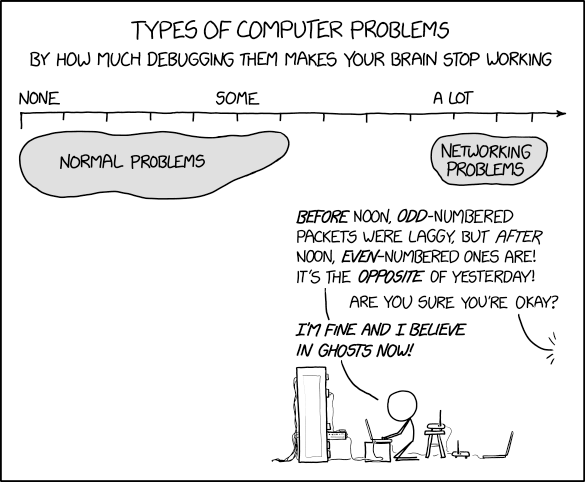
\includegraphics[width=0.9\linewidth]{xkcd.png}
\end{center}

\end{multicols*}

\end{document}